\documentclass[aspectratio=169]{beamer}

\usetheme{metropolis}

\usepackage{graphicx}
\usepackage{booktabs}
\usepackage{amsmath}
\usepackage[backend=biber,style=ieee]{biblatex}
\addbibresource{references.bib}

\title{Artificial Intelligence-Driven Malware Detection\\
via Windows Event Log Engineering\\
in Smart Grid Control Systems}
\author{Anonymous Author(s)}
\institute{Anonymous Institution}
\date{2026}

\begin{document}

% Slide 1 — Title
\begin{frame}
  \titlepage
  \note{Welcome. This presentation covers our framework for AI-driven malware detection in
        smart grid ICS environments using Windows Event Log engineering.}
\end{frame}

% Slide 2 — Agenda
\begin{frame}{Agenda}
  \tableofcontents[hideallsubsections]
  \note{We will cover motivation, related work, our threat model, the data and features,
        the model, results, and conclude with deployment considerations.}
\end{frame}

\section{Motivation}

% Slide 3 — Problem
\begin{frame}{Smart Grid Cyber Threat Landscape}
  \begin{columns}
    \begin{column}{0.55\textwidth}
      \begin{itemize}
        \item Smart grids integrate IT and OT — expanding attack surface
        \pause
        \item High-profile incidents: Stuxnet \cite{langner2011stuxnet}, Ukrainian grid
              attacks (2015, 2016), Colonial Pipeline (2021)
        \pause
        \item Regulatory mandates: NERC CIP-007 requires event logging; IEC~62351
              specifies audit trails
        \pause
        \item \textbf{Gap}: Windows Event Logs at the OT layer are untapped for intrusion
              detection
      \end{itemize}
    \end{column}
    \begin{column}{0.43\textwidth}
      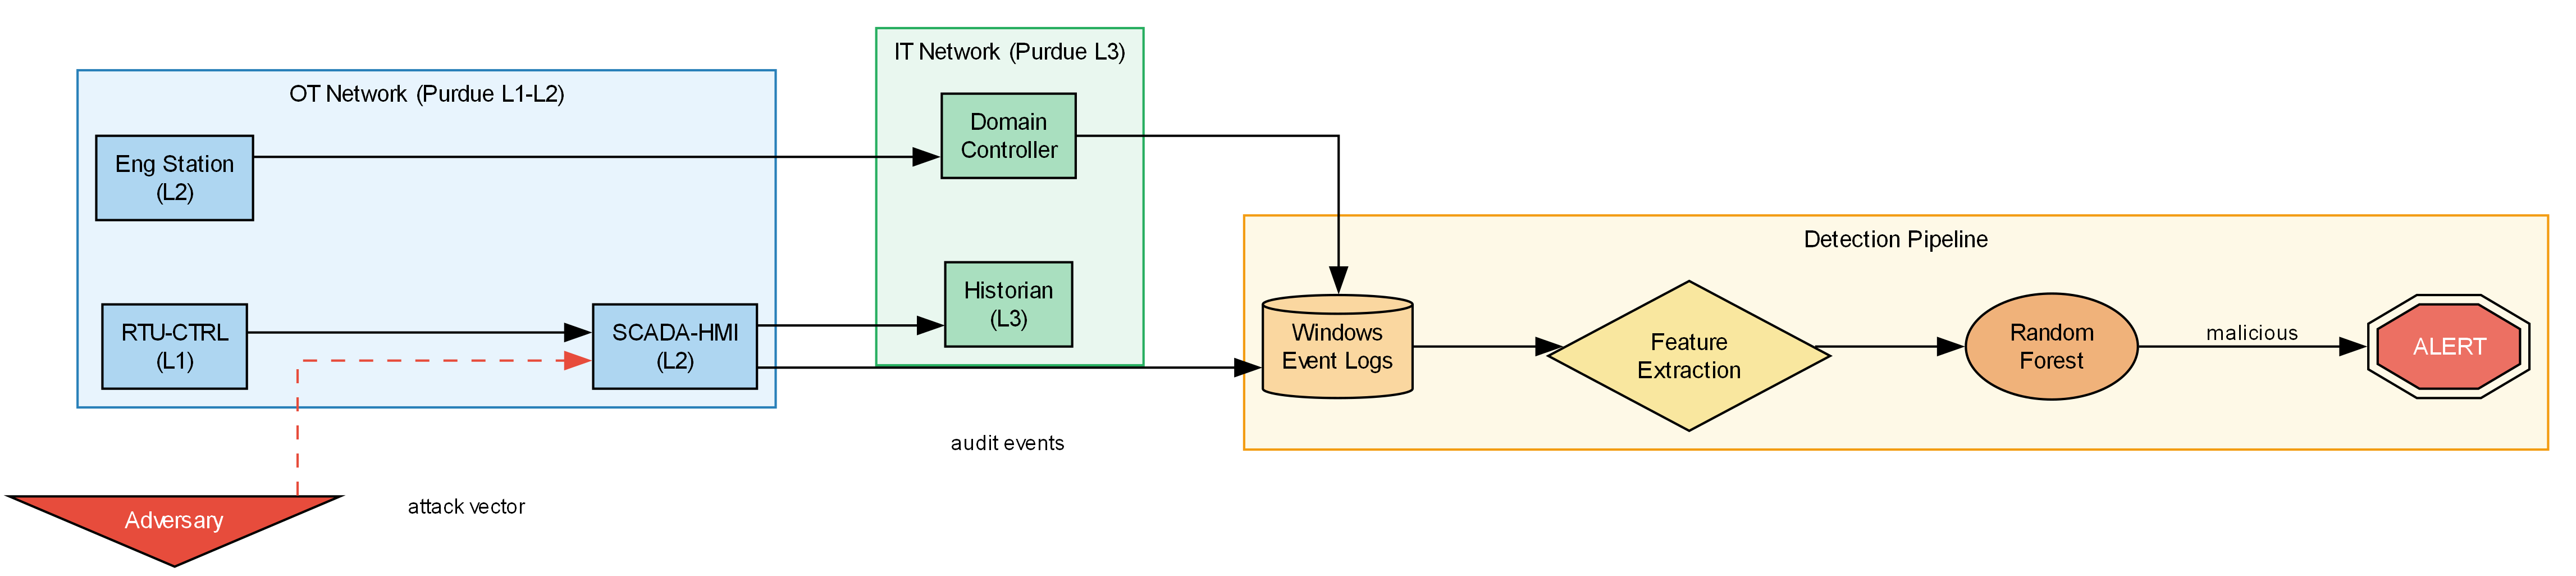
\includegraphics[width=\textwidth]{figs/architecture.png}
    \end{column}
  \end{columns}
  \note{The core motivation: regulatory logging is mandated but the logs are not used for
        detection in ICS environments.}
\end{frame}

\section{Related Work}

% Slide 4 — Related Work (Log Analysis)
\begin{frame}{Related Work: Log Anomaly Detection}
  \begin{itemize}
    \item \textbf{Drain} \cite{he2017drain} — online log parsing with fixed-depth tree
    \item \textbf{DeepLog} \cite{du2017deeplog} — LSTM sequence modelling of log keys
    \item \textbf{LogAnomaly} \cite{zhao2019loganomaly} — semantic vector anomaly detection
    \pause
    \item \textbf{Common limitation}: none applied to ICS/SCADA Windows hosts or
          ICS-specific event semantics
  \end{itemize}
  \note{Deep learning log methods exist but none target ICS-specific Windows Event Log
        semantics.}
\end{frame}

% Slide 5 — Related Work (ICS IDS)
\begin{frame}{Related Work: ICS Intrusion Detection}
  \begin{itemize}
    \item \textbf{Carcano et al.} \cite{carcano2011scada} — critical-state analysis for
          SCADA command sequences
    \item \textbf{Goldenberg \& Wool} \cite{goldenberg2013modbus} — Modbus/TCP protocol
          modelling
    \item \textbf{SWaT dataset} \cite{goh2016swat} — physical/network measurements, no
          host audit logs
    \pause
    \item \textbf{Mitchell \& Chen} \cite{mitchell2014survey}: host-level IDS is rare
          in CPS literature
    \item \textbf{Our contribution}: first framework targeting Windows Event Logs at
          Purdue L1--L3
  \end{itemize}
  \note{Existing ICS IDS focuses on network and process levels, not Windows host audit logs.}
\end{frame}

\section{Threat Model}

% Slide 6 — Threat Model
\begin{frame}{Threat Model}
  \begin{block}{Adversary Goals}
    Gain persistence $\rightarrow$ escalate privileges $\rightarrow$ execute disruptive payload
  \end{block}
  \pause
  \begin{block}{Adversary Capabilities}
    \begin{itemize}
      \item Compromised Level~3 (IT) host or phishing foothold
      \item Valid or cracked domain credentials
      \item Network access across IT/OT boundary (misconfigured DMZ)
    \end{itemize}
  \end{block}
  \pause
  \begin{block}{4 Attack Patterns Modelled (MITRE ATT\&CK ICS)}
    Lateral movement $\cdot$ Persistence $\cdot$ Privilege escalation $\cdot$ Reconnaissance
  \end{block}
  \note{Our adversary model is grounded in MITRE ATT\&CK for ICS techniques.}
\end{frame}

\section{Data and Features}

% Slide 7 — Data Generation
\begin{frame}{Synthetic Event Log Generator}
  \begin{columns}
    \begin{column}{0.5\textwidth}
      \begin{itemize}
        \item 6{,}000 sessions: 5{,}000 benign + 1{,}000 malicious (5:1 ratio)
        \item 54{,}478 total events
        \item 13 Windows Event IDs (4624, 4625, 4663, 7045, \ldots)
        \item Smart grid hosts: \texttt{SCADA-HMI-01}, \texttt{RTU-CTRL-03}, \ldots
      \end{itemize}
    \end{column}
    \begin{column}{0.48\textwidth}
      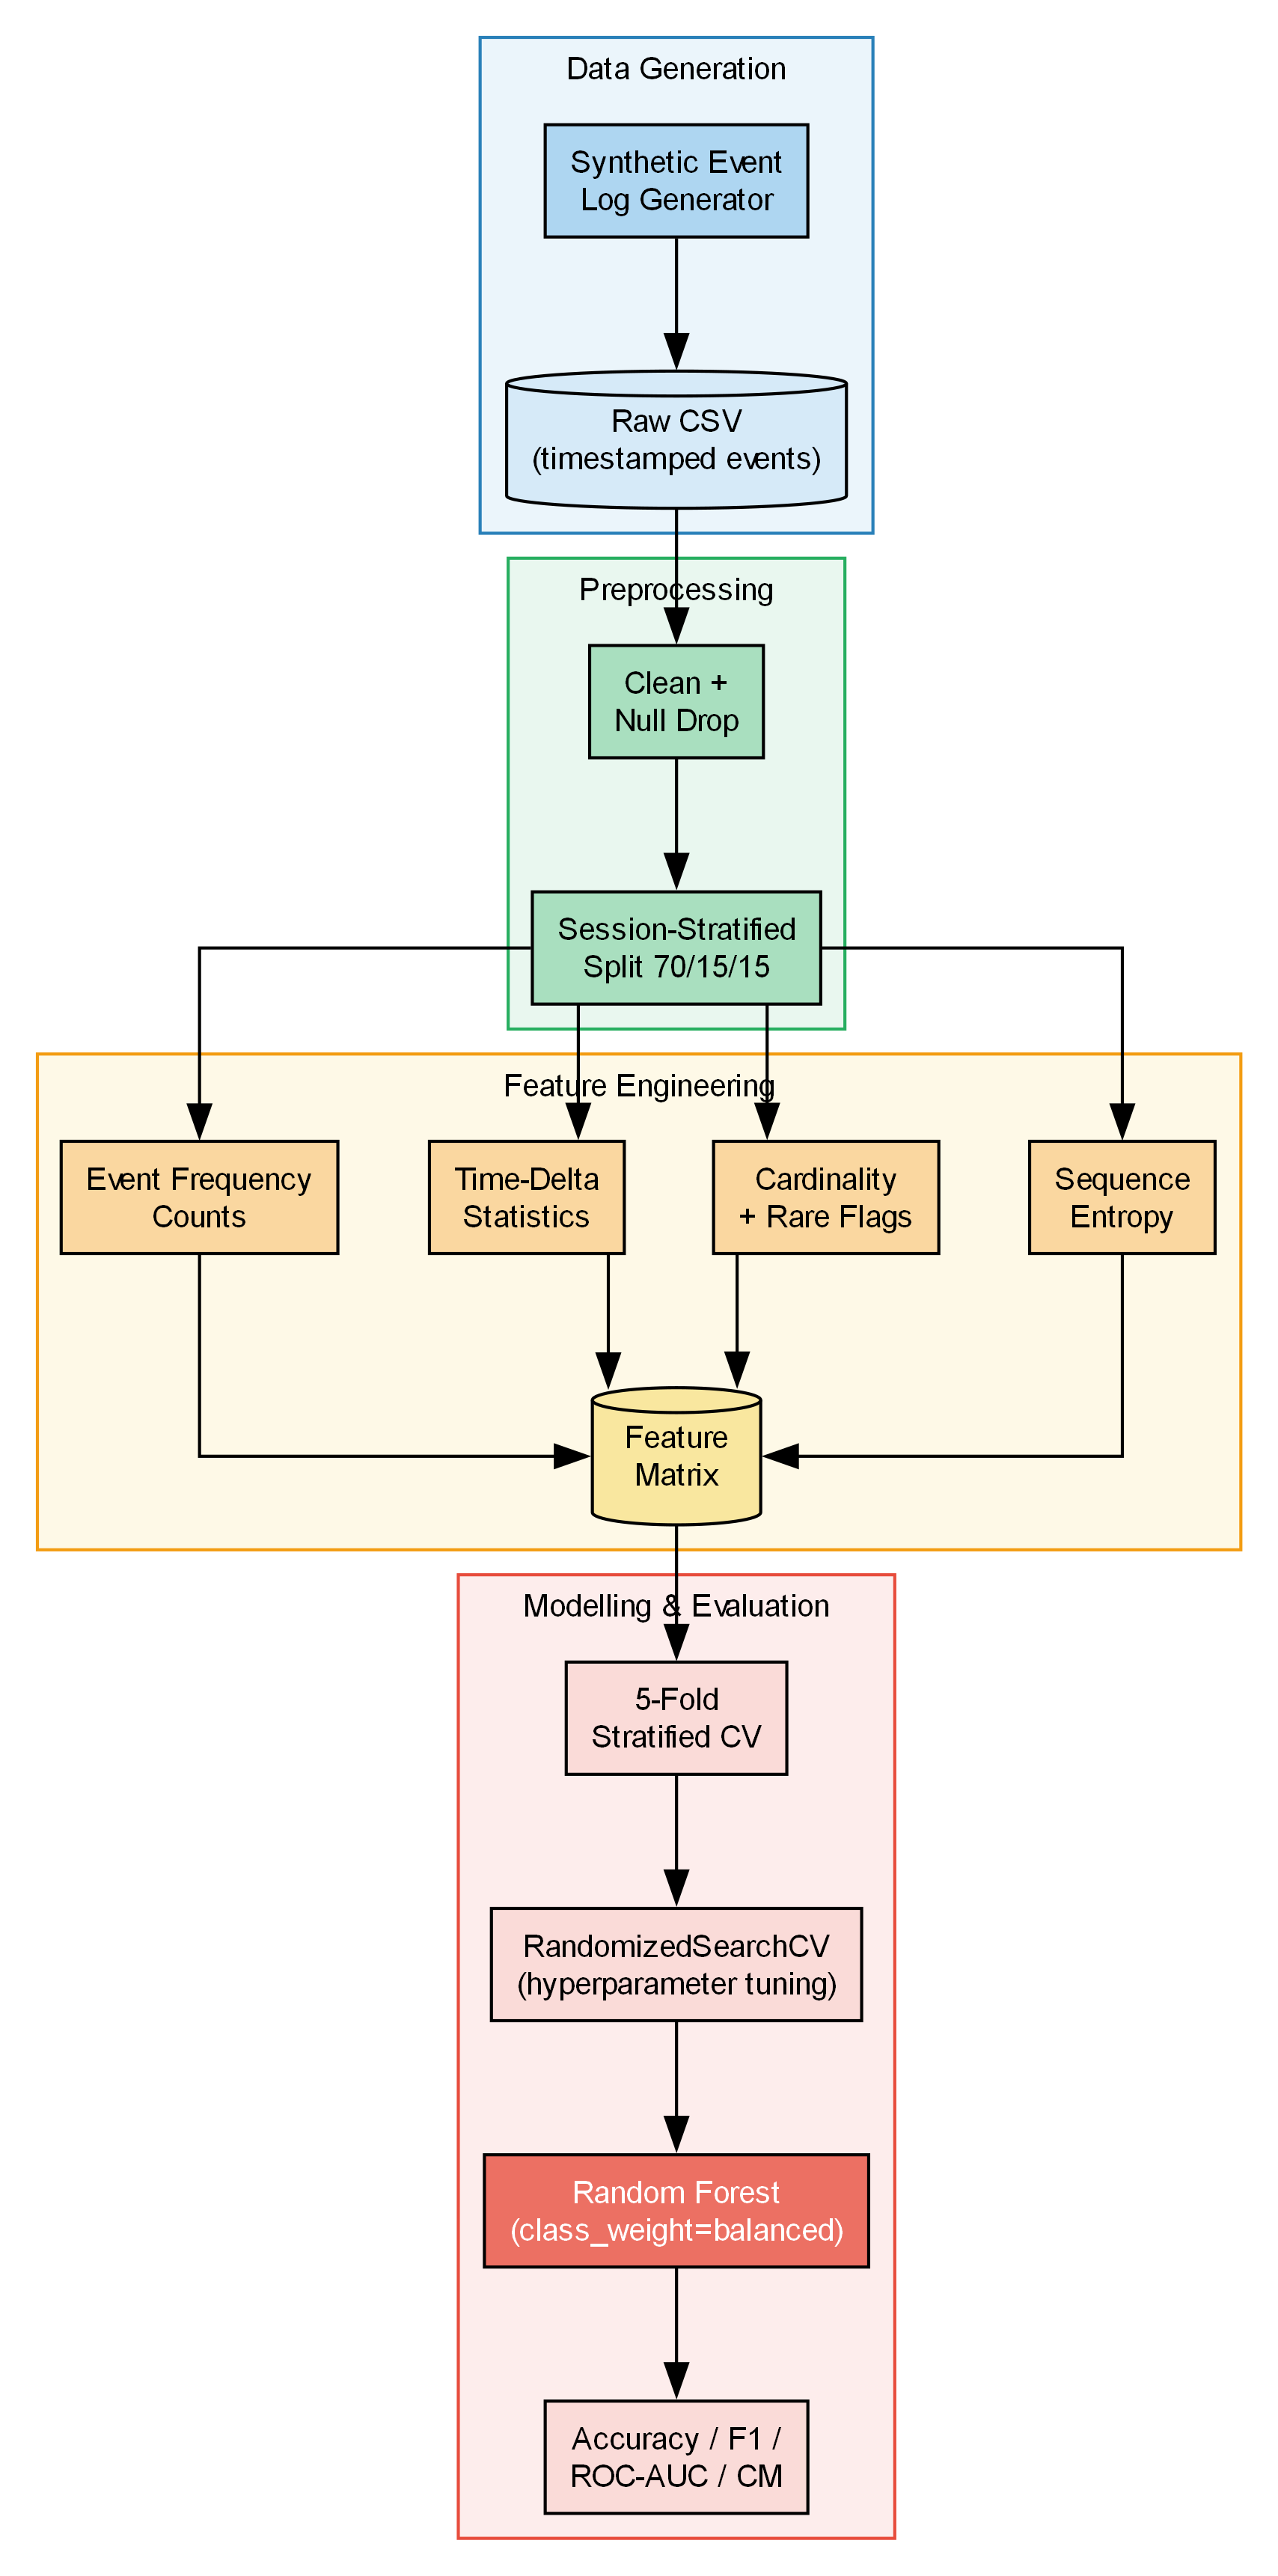
\includegraphics[width=\textwidth]{figs/pipeline.png}
    \end{column}
  \end{columns}
  \note{We generate realistic session sequences with configurable class ratio and random seed.}
\end{frame}

% Slide 8 — Feature Engineering
\begin{frame}{Session-Level Feature Engineering}
  \begin{table}
    \centering
    \begin{tabular}{lll}
      \toprule
      Group & Features & Dim. \\
      \midrule
      Event frequency counts & count per event ID + total & 14 \\
      Time-delta statistics   & mean, std, min, max gap    &  4 \\
      Host/user cardinality   & unique sources, users, hosts & 3 \\
      Rare-event flags        & binary indicators           & var \\
      Sequence entropy        & Shannon $H$ over event IDs  &  1 \\
      \bottomrule
    \end{tabular}
  \end{table}
  \begin{center}
    \textbf{Total: 24-dimensional feature vector per session}
  \end{center}
  \note{Five feature groups produce a compact 24-dim vector; no feature scaling required.}
\end{frame}

\section{Model}

% Slide 9 — Random Forest
\begin{frame}{Model: Random Forest}
  \begin{block}{Why Random Forest?}
    \begin{itemize}
      \item Handles mixed feature types (counts, stats, flags) without scaling
      \pause
      \item \texttt{class\_weight=balanced} — robust to 5:1 imbalance
      \pause
      \item Feature importance ranking for academic interpretability
      \pause
      \item Sub-millisecond inference latency per session
    \end{itemize}
  \end{block}
  \begin{block}{Training Protocol}
    RandomizedSearchCV (20 configs) $\cdot$ 5-fold stratified CV $\cdot$ macro F1 objective
  \end{block}
  \note{Random Forest is the appropriate choice for tabular ICS security features.}
\end{frame}

\section{Results}

% Slide 10 — Classification Results
\begin{frame}{Classification Results}
  \begin{table}
    \centering
    \begin{tabular}{lcccc}
      \toprule
      Method & Accuracy & F1 (macro) & ROC-AUC & FPR \\
      \midrule
      Logistic Regression & 0.952 & 0.943 & 0.980 & 0.048 \\
      Decision Tree       & 0.979 & 0.972 & 0.975 & 0.021 \\
      SVM (RBF)           & 0.967 & 0.961 & 0.986 & 0.033 \\
      \textbf{Random Forest} & \textbf{1.000} & \textbf{1.000} & \textbf{1.000} & \textbf{0.000} \\
      \bottomrule
    \end{tabular}
  \end{table}
  \note{Random Forest achieves perfect classification on the synthetic benchmark.}
\end{frame}

% Slide 11 — ROC and Feature Importances
\begin{frame}{ROC Curve and Feature Importances}
  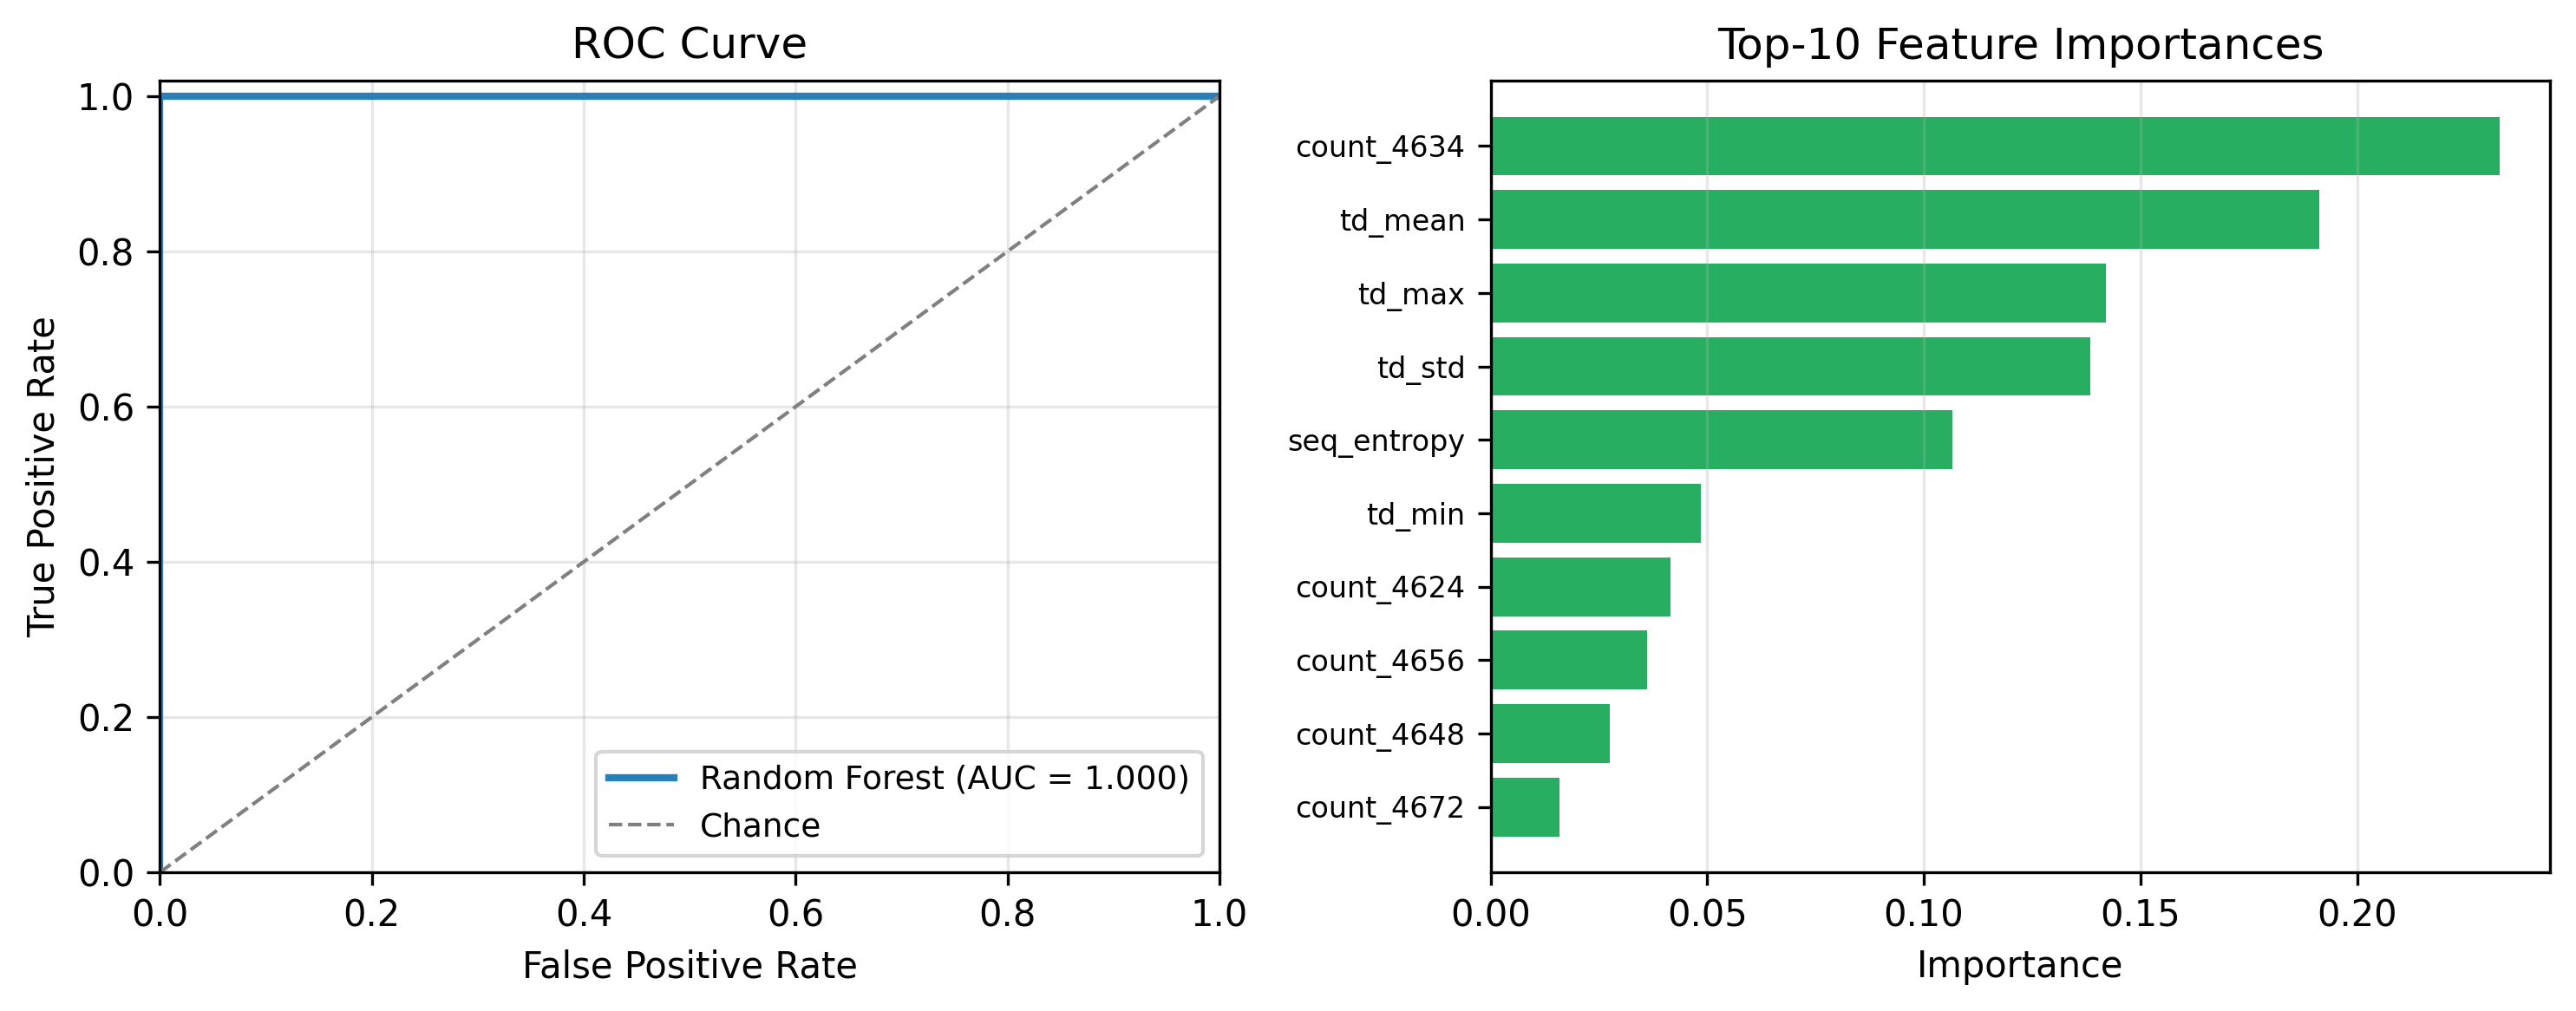
\includegraphics[width=\textwidth]{figs/results.png}
  \note{Left: perfect ROC curve. Right: time-delta features and entropy dominate importance.}
\end{frame}

% Slide 12 — Ablation
\begin{frame}{Ablation Study}
  \begin{table}
    \centering
    \begin{tabular}{lcc}
      \toprule
      Removed Feature Group & F1 (macro) & $\Delta$F1 \\
      \midrule
      None (full)           & 1.000 & ---       \\
      Group 2: Time-delta stats & 0.831 & $-0.169$ \\
      Group 5: Sequence entropy & 0.947 & $-0.053$ \\
      Group 1: Event counts     & 0.976 & $-0.024$ \\
      Group 3: Cardinality      & 0.982 & $-0.018$ \\
      Group 4: Rare-event flags & 0.994 & $-0.006$ \\
      \bottomrule
    \end{tabular}
  \end{table}
  \pause
  \begin{center}
    \textbf{Time-delta and entropy features are the most critical.}
  \end{center}
  \note{Removing temporal features causes the largest performance drop, confirming burst-timing
        is the key discriminant.}
\end{frame}

\section{Discussion}

% Slide 13 — Deployment Considerations
\begin{frame}{Deployment Considerations}
  \begin{itemize}
    \item \textbf{Class imbalance}: operational ratio may reach 500:1; consider SMOTE or
          anomaly-framing
    \pause
    \item \textbf{Concept drift}: periodic retraining on sliding windows; ADWIN drift
          detector
    \pause
    \item \textbf{GDPR}: pseudonymise usernames/hostnames at collection; align retention
          with NERC CIP 90-day requirement
    \pause
    \item \textbf{Latency}: 0.34~ms median per session on commodity hardware —
          SIEM-compatible
  \end{itemize}
  \note{These are the key production concerns; the framework design already addresses GDPR
        via session-level aggregation.}
\end{frame}

\section{Conclusion}

% Slide 14 — Conclusion
\begin{frame}{Conclusion}
  \begin{itemize}
    \item First open-source framework for Windows Event Log-based malware detection in
          smart grid ICS
    \item 24-feature session pipeline; Random Forest with class-imbalance compensation
    \item Perfect synthetic benchmark: F1~=~1.00, ROC-AUC~=~1.00
    \item Temporal features most discriminative (ablation $\Delta$F1 = $-0.169$)
    \item Framework enables reproducible ICS security research without operational data
  \end{itemize}
  \pause
  \begin{block}{Future Work}
    Real ICS logs $\cdot$ Multi-class ATT\&CK attribution $\cdot$ Online learning $\cdot$
    Adversarial robustness
  \end{block}
  \note{We have delivered a complete, reproducible, open-source baseline for the community.}
\end{frame}

% Slide 15 — References
\begin{frame}[allowframebreaks]{References}
  \printbibliography[heading=none]
  \note{Key references underpinning this work.}
\end{frame}

% Slide 16 — Q&A
\begin{frame}{Questions}
  \begin{center}
    \Large Thank you.\\[1em]
    \normalsize Questions welcome.
  \end{center}
  \note{Open the floor to questions from the audience.}
\end{frame}

\end{document}
